% P05 diagnostic figure reliability_bins|held_evaluation|M01; allowlisted public aggregate points.
% Each point is an aggregate mean or bin over repeated contexts, not an independent sample.
% data_sha256=7f60e425b5fe235c362c21442c3237e1521aad33df8bebdebfd5854e0cfadd4b
\documentclass[tikz,border=5pt]{standalone}
\ifdefined\pdfinfoomitdate\pdfinfoomitdate=1\fi
\ifdefined\pdfsuppressptexinfo\pdfsuppressptexinfo=-1\fi
\ifdefined\pdftrailerid\pdftrailerid{}\fi
\usepackage{pgfplots}
\usepgfplotslibrary{groupplots}
\pgfplotsset{compat=1.18}
\definecolor{p05Blue}{HTML}{0072B2}
\definecolor{p05Orange}{HTML}{E69F00}
\definecolor{p05Green}{HTML}{009E73}
\definecolor{p05Purple}{HTML}{CC79A7}
\definecolor{p05Red}{HTML}{D55E00}
\definecolor{p05Sky}{HTML}{56B4E9}
\begin{document}
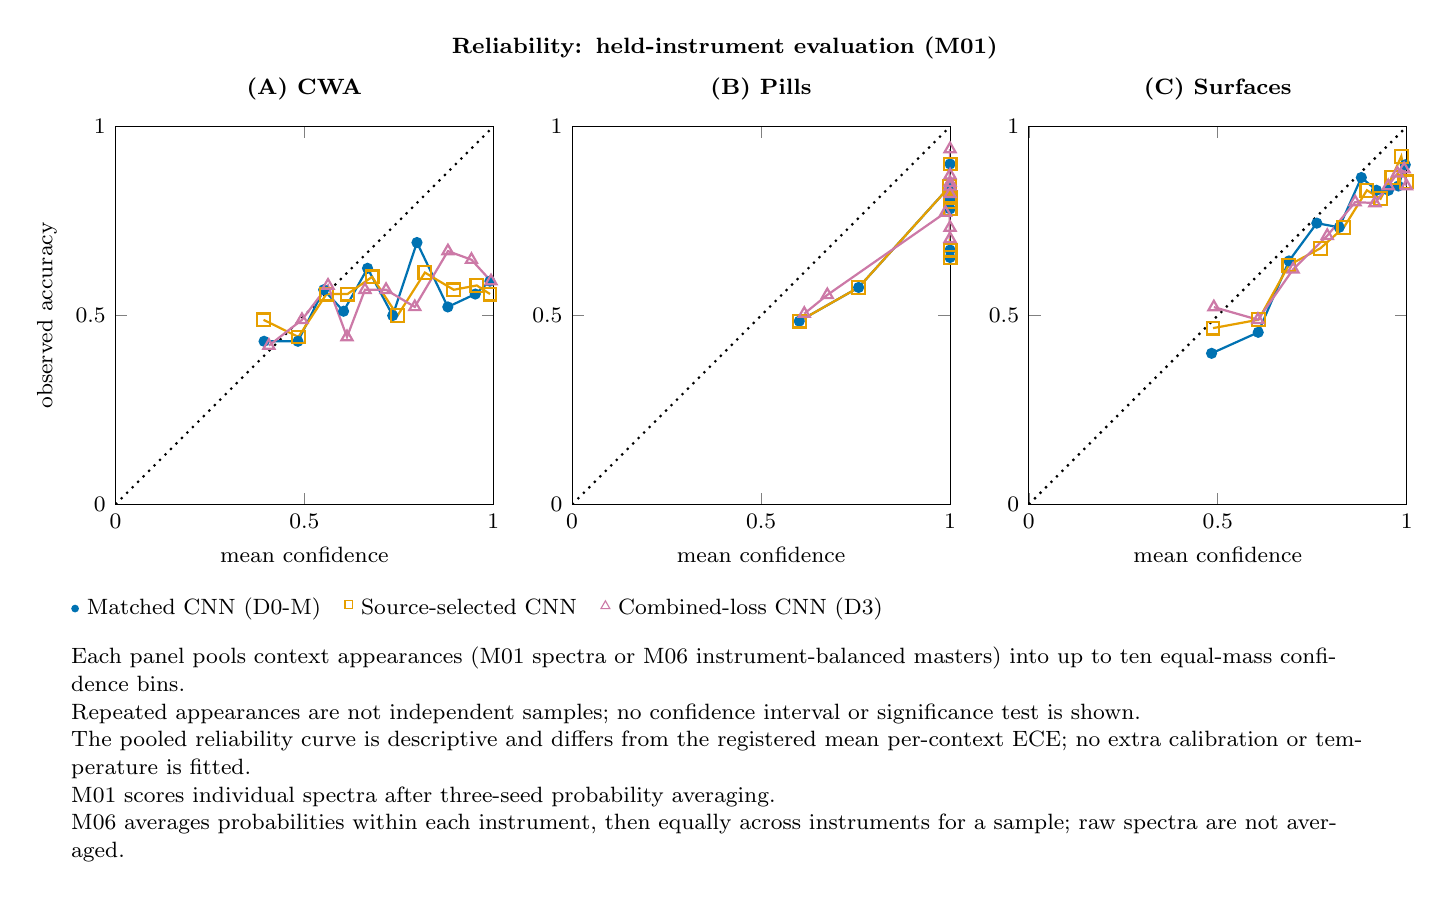
\begin{tikzpicture}
\begin{groupplot}[
  group style={group size=3 by 1, horizontal sep=1.0cm, vertical sep=1.8cm},
  width=4.8cm, height=4.8cm, scale only axis,
  xmin=0, xmax=1, ymin=0, ymax=1,
  xtick={0,0.5,1}, ytick={0,0.5,1},
  tick label style={font=\fontsize{8}{10}\selectfont, color=black},
  label style={font=\fontsize{8}{10}\selectfont, color=black},
  title style={font=\fontsize{8}{10}\selectfont\bfseries, color=black},
]
\nextgroupplot[title={(A) CWA}, xlabel={mean confidence}, ylabel={observed accuracy}]
\addplot[black, dotted, line width=0.8pt] coordinates {(0,0) (1,1)};
\addplot[mark=*, mark size=1.6pt, color=p05Blue, line width=0.8pt, mark options={fill=p05Blue, draw=p05Blue}] coordinates {(0.39333652994825719,0.43181818181818182) (0.48290448296241661,0.43181818181818182) (0.55111254237678309,0.56818181818181823) (0.60369135606343527,0.51136363636363635) (0.66709005655643994,0.625) (0.73369619547679865,0.5) (0.79785339877606143,0.69318181818181823) (0.87946392740180312,0.52272727272727271) (0.95214696915423613,0.55681818181818177) (0.99079169806516953,0.59090909090909094)};
\addplot[mark=square, mark size=2.3pt, color=p05Orange, line width=0.8pt, mark options={fill=none, draw=p05Orange}] coordinates {(0.39204020369555831,0.48863636363636365) (0.48405268429322967,0.44318181818181818) (0.55837258330470463,0.55681818181818177) (0.61395687020175849,0.55681818181818177) (0.67921629972519937,0.60227272727272729) (0.74652805632578989,0.5) (0.81886080473609435,0.61363636363636365) (0.89509425996247127,0.56818181818181823) (0.95622719950016977,0.57954545454545459) (0.99109532343855766,0.55681818181818177)};
\addplot[mark=triangle, mark size=2.3pt, color=p05Purple, line width=0.8pt, mark options={fill=none, draw=p05Purple}] coordinates {(0.40603119578766511,0.42045454545454547) (0.49357436551177519,0.48863636363636365) (0.56247711862367966,0.57954545454545459) (0.61273560560492157,0.44318181818181818) (0.66027996096807162,0.56818181818181823) (0.71604924358271616,0.56818181818181823) (0.79219124424627685,0.52272727272727271) (0.87979953001130617,0.67045454545454541) (0.94201446693387225,0.64772727272727271) (0.99379896095548725,0.59090909090909094)};
\nextgroupplot[title={(B) Pills}, xlabel={mean confidence}]
\addplot[black, dotted, line width=0.8pt] coordinates {(0,0) (1,1)};
\addplot[mark=*, mark size=1.6pt, color=p05Blue, line width=0.8pt, mark options={fill=p05Blue, draw=p05Blue}] coordinates {(0.60103200876581631,0.48514851485148514) (0.7580376619662812,0.57425742574257421) (0.99910817903769689,0.84158415841584155) (0.99999998897603715,0.81188118811881194) (0.99999999999999944,0.90099009900990101) (1,0.67326732673267331) (1,0.80198019801980203) (1,0.78217821782178221) (1,0.65346534653465349) (1,0.81188118811881194)};
\addplot[mark=square, mark size=2.3pt, color=p05Orange, line width=0.8pt, mark options={fill=none, draw=p05Orange}] coordinates {(0.60103200876581631,0.48514851485148514) (0.7580376619662812,0.57425742574257421) (0.99910817903769689,0.84158415841584155) (0.99999998897603715,0.81188118811881194) (0.99999999999999944,0.90099009900990101) (1,0.67326732673267331) (1,0.80198019801980203) (1,0.78217821782178221) (1,0.65346534653465349) (1,0.81188118811881194)};
\addplot[mark=triangle, mark size=2.3pt, color=p05Purple, line width=0.8pt, mark options={fill=none, draw=p05Purple}] coordinates {(0.6142759972319366,0.50495049504950495) (0.67522057633919985,0.5544554455445545) (0.98774417250050162,0.7722772277227723) (0.9999999978280445,0.82178217821782173) (1,0.87128712871287128) (1,0.73267326732673266) (1,0.85148514851485146) (1,0.94059405940594054) (1,0.70297029702970293) (1,0.84158415841584155)};
\nextgroupplot[title={(C) Surfaces}, xlabel={mean confidence}]
\addplot[black, dotted, line width=0.8pt] coordinates {(0,0) (1,1)};
\addplot[mark=*, mark size=1.6pt, color=p05Blue, line width=0.8pt, mark options={fill=p05Blue, draw=p05Blue}] coordinates {(0.4836451099854725,0.40000000000000002) (0.60701484422356577,0.45555555555555555) (0.688441100841099,0.64444444444444449) (0.76204754531488605,0.74444444444444446) (0.82133162887528388,0.73333333333333328) (0.87990222745045654,0.8651685393258427) (0.91979602669964977,0.8314606741573034) (0.95177975011723193,0.8314606741573034) (0.97790728729288368,0.84269662921348309) (0.99609048790477672,0.898876404494382)};
\addplot[mark=square, mark size=2.3pt, color=p05Orange, line width=0.8pt, mark options={fill=none, draw=p05Orange}] coordinates {(0.48741890337715338,0.46666666666666667) (0.60771992201883018,0.48888888888888887) (0.68794994526968867,0.6333333333333333) (0.77141216572661953,0.67777777777777781) (0.83369276142027837,0.73333333333333328) (0.89458359606268867,0.8314606741573034) (0.93069998048638769,0.8089887640449438) (0.96045785500366732,0.8651685393258427) (0.98561330303458417,0.9213483146067416) (0.99870210404704285,0.8539325842696629)};
\addplot[mark=triangle, mark size=2.3pt, color=p05Purple, line width=0.8pt, mark options={fill=none, draw=p05Purple}] coordinates {(0.48965523009318329,0.52222222222222225) (0.60625556819888815,0.48888888888888887) (0.69932039796535839,0.62222222222222223) (0.78968259844940281,0.71111111111111114) (0.86345324327914008,0.80000000000000004) (0.9157394420001187,0.797752808988764) (0.95100175737956349,0.84269662921348309) (0.97521203571191961,0.8764044943820225) (0.99303676468726754,0.88764044943820219) (0.99933291940855484,0.84269662921348309)};
\end{groupplot}
\node[anchor=south, font=\fontsize{8}{10}\selectfont\bfseries, color=black, align=center, text width=16.6cm] at (current bounding box.north) {Reliability: held-instrument evaluation (M01)};
\node[anchor=north, font=\fontsize{8}{10}\selectfont, color=black, align=left, text width=16.6cm] (p05legend) at ([yshift=-2mm]current bounding box.south) {\tikz[baseline=-0.6ex]\fill[p05Blue](0,0)circle(1.4pt);\ Matched CNN (D0-M)\quad \tikz[baseline=-0.6ex]\draw[p05Orange](0,0)rectangle(2.8pt,2.8pt);\ Source-selected CNN\quad \tikz[baseline=-0.6ex]\draw[p05Purple](0,0)--(1.6pt,2.8pt)--(3.2pt,0)--cycle;\ Combined-loss CNN (D3)};
\node[anchor=north, font=\fontsize{8}{10}\selectfont, color=black, align=left, text width=16.6cm] at ([yshift=-1mm]p05legend.south) {Each panel pools context appearances (M01 spectra or M06 instrument-balanced masters) into up to ten equal-mass confidence bins.\\Repeated appearances are not independent samples; no confidence interval or significance test is shown.\\The pooled reliability curve is descriptive and differs from the registered mean per-context ECE; no extra calibration or temperature is fitted.\\M01 scores individual spectra after three-seed probability averaging.\\M06 averages probabilities within each instrument, then equally across instruments for a sample; raw spectra are not averaged.};
\end{tikzpicture}
\end{document}
